%!TEX root = ../../thesis.tex
%!TEX enableSynctex = true
%*******************************************************************************
%****************************** Third Chapter **********************************
%*******************************************************************************
% **************************** Define Graphics Path **************************
\ifpdf
    \graphicspath{{Chapters/dualslit/Figs/Raster/}{Chapters/dualslit/Figs/PDF/}{Chapters/dualslit/Figs/}}
\else
    \graphicspath{{Chapters/dualslit/Figs/Vector/}{Chapters/dualslit/Figs/}}
\fi

\chapter{Developments in confocal virtual slit-scanning microscopy}

%Confocal microscopy is a variant of a pointing scanning systems whereby a pin hole in a conjugate plane rejects out-of-focus light to enable volumetric imaging.
%Similarly a slit may replace a pinhole greatly speeding up the acquisition process for the cost of resolution and %sectioning capabilities.
%In digitially scanned light-sheet microscopy, the swept beam may be conjugated to a slit to provide better contrast, resolution and sectioning in the direction of scanning.

Conventional epi-illumination fluorescence microscopes illuminate the focal plane of the detection objective as well as a large fraction of the sample outside the focal plane.
This leads to background intensity due to out-of-focus fluorescence, affecting resolution and contrast.
Confocal-microscopes use a pin-hole in a conjugate image plane to forcibly reject fluorescence from outside of the focal plane, producing overall better axially resolved images and contrast and resolution.
Sectioning by this means leads to a large photon dose throughout the sample and with a cost to overall speed.
Light-sheet microscopes address this generally by illuminating with a \emph{thin} sheet of light orthogonally to the sample; but for having wide-field contrast and optical sectioning being on the order of the thickness of the light-sheet.

\section{Single beam confocal slit-scanning}

It was shown that a confocal microscope may be run faster by using a narrow slight rather than a pin-hole, this increased contrast and resolution in one direction only.
The same principle can be applied to a digitally scanned light-sheet, provided the propagation of the beam is in the same direction of the slit.
By scanning the slit and the beam concomitantly, an increase in resolution and contrast may be achieved in one direction.
Moreover, the out-of-focus light now being rejected then increases the overall axial resolution in one imaging axis.

There exist several approaches for the implementation of such a confocal slit system.
The simplest approach is to add a slit in the conjugate image plane and synchronously shift the slit with the scanning illumination.
The forces involved in accelerating a slit would be large as the slit would be moving at \SI{\sim 10}{\kilo\hertz} linearly.
A more practical approach would involve de-scanning the entire image onto a static slit using galvanometric mirrors.
This does introduce more complexity to a system, but has the potential to increase the overall available field of view beyond just the field number of the detection objective \cite{Huisken}.
This technique was exploited to great effect by Huisken \emph{et. al.} whereby they used descanning to keep the emission photons of the beam along one row of pixels on a camera.
they then filled the rest of the chip with spectral information by placing a diffractive element in emission path \cite{}.

%Physical slits may be substituted for virtual slits when exploiting the nature of sCMOS cameras.
By selectively activating pixels on an sCMOS detector for read-off, out-of-focus light may be rejected in a similar fashion to a real slit.
%The process of rolling a shutter occurs within the electronics of the camera for pixel read off by design.
The rolling of the shutter with the concomitant sweeping of the beam of light allows for live confocal imaging is (Fig. \ref{fig:slit_scanning_alt}).
The width of the slit adjusts the contrast and resolution of the final image, where an optimal SNR should be when the slit is of a similia.r
Setting the width of the rolling slit to be similar to the width of the light beam
Controlling the width of the slit to near the width of the beam,

\begin{figure}
  \centering
  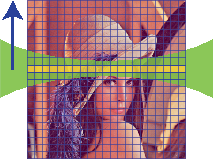
\includegraphics{slit_scanning_alt}
  \caption{The principle of confocal slit scanning using digital light-sheet microscopy.
  An incident beam (green) approaches orthogonally to the direction of the rolling shutter, the shutter consists of a width of active pixels (yellow).
  The inactive pixels correspond to out-of-focus light and are rejected from the final image.}
  \label{fig:slit_scanning_alt}
\end{figure}

\subsection{Implementation}

%Talk about synchornisaiton

\todonotes{Talk about the implementation and synchronisation (boring)}


\subsection{Optimisation}

A characterisation of the optimal slit width of the virtual slit was needed to provide maximal imaging contrast.
To measure this, \SI{200}{\nano\metre} fluorescent beads were suspended in 1\% agarose VII gel at a concentration of [insert concentration]. %%~2.3 × 1010 particles/mL
The agarose was mounted by pipetting on warm to an lightly scratched PDMS bar, this helped adherence.
Entire volumes (2048 $\times$ 2048 $\times$ \SI{100}{\micro\metre}) were imaged per each slit width varied.
Beads were then localised manually through a axially projected image (see Chapter \ref{sec:} %TODO insert chapter
).

\SI{31} were localised with a single candidate bead that was suitable as it was not part of an aggregate, it was sufficiently bright and unobscured.
By analysing both the SNR and the contrast of each cropped window around the candidate bead it was shown that the ideal slit width was \SI{2.51(5)}{\micro\metre} which is on the order of the width of the incident laser beam, \SI{2.3(2)}{\micro\metre} (Fig. \ref{fig:optimal_slit_snr_contrast}).
%Beam width 18 pixels. 2048 pixels, 25x mag each pixel 502 um
The SNR was evaluated by computing the ratio of its summed squared magnitude to that of the noise.
The contrast was calculated by fitting a 2D Gaussian to each bead image and plotting the fitted amplitude $A$, from:

\begin{align}
  A e^{-\left(\frac{(x-x_0)^2-(y-y_0)^2}{2\sigma^2}\right)}
\end{align}

\begin{figure}
  \centering
  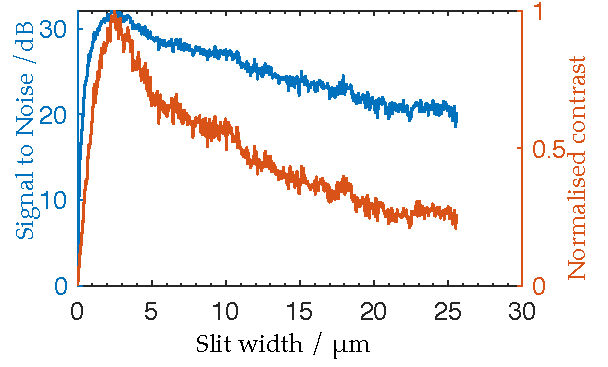
\includegraphics{Chapters/dualslit/Figs/PDF/optimal_slit_snr_contrast}
  \caption{Optimising the confocal slit width by varying slit width on a single fluorescent bead}
  \label{fig:optimal_slit_snr_contrast}
\end{figure}


%\section{Implementation}

%Galvo mirror and virtual Slit
%Galvo mirror and static slit with relay optics and de-scanning unit
%Galvo mirror and fast actuator

%Using a virtual slit requires precise synchronisation.
%Need an initial delay, as sCMOS chip used here requires a 10ms period to initialise electronics.
%During this period the Galvo can be pre-driven so that the velocity is linear once the exposure begins
%The galvo is then sinusoidally returned at the end of the exposure.

%\subsection{Slit-descanning} %Huisken did this in hyperspectral paper
%\subsection{Improvement} %Could use fran's results or repeat mine (rather latter)

%\subsection{Limitations} %Show that mismatch between beam and slit xy is bad and z is bad
\section{Double speed slit-scanning microscopy}

The sensor used in the Orca Flash v4 (as well as other sCMOS cameras including the Pco.Edge and Andor Zyla) consists of two adjacent Fairchild sCMOS chips.
In global shutter mode a shutter will propagate outwards from the centre of the chip simultaneously and in the fastest exposure possible for each chip (10ms), this provides the maximum \SI{100}{\hertz} imaging.
For confocal slit scanning the chips are addressed serially with a single thin shutter propagating from one side of the sensor to the other.
In this mode the maximum frame rate achievable is \SI{50}{\hertz} when scanning confocally.

In this work a custom camera firmware was used to enable a pair of confocal slits to scan simultaneously providing the \SI{100}{\hertz} that was ordinarily available in global shutter mode.

\begin{figure}
  \centering
  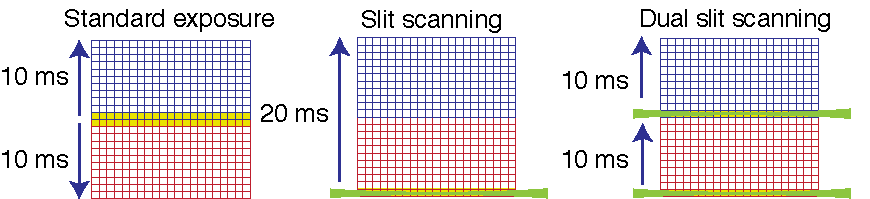
\includegraphics{dual_slit_scanning}
  \caption{
  Principle behind doubling the frame rate of the Orca Flash v4 when using slit scanning mode.
  Standard exposure: In global shutter mode \SI{100}{\hertz} imaging may be achieved as each side of the sensor rolls an independent shutter.
  Slit scanning: In normal slit scanning mode the shutter moves from one half of the chip to the other serially, halving available framerate.
  Dual-slit scanning:
  The full frame-rate of the sensor is achievable when using two rolling shutters
  %Having two shutters roll in slit scanning
  %Having two shutters roll in slit scanning mode would make available the full of frame rate
  }
  \label{fig:dual_slit_scanning}
\end{figure}

\subsection{Dual-beam implementation}
\subsubsection{SLM}
Initially an SLM was imaged directly onto the first scanning mirror using a relay pair of lenses (Fig. \ref{fig:dual_beam_layouts} a); the relay at the scan mirror allowed access to the image plane of the scan mirror, whilst the second relay controlled the pixel size of the SLM at the imaging plane of the excitation objective.
This implementation was polarisation sensitive and caused difficult for distributing an equal amount of power into each beam, due to the discrete nature of the voltage being applied to each SLM pixel.
Due to the pixel nature of the SLM as well the separation of the two beams could only be discrete distances with the step size being larger than a single pixel at the detector.
Using SLMs also limited the potential for creating exotic illumination superimposed on the dual beams.
Thought solutions to exist (using super-pixels\cite{}, or dual SLMs \cite{}) the methods are limited and heavily heavily optically involved.

\begin{figure}
  \centering
  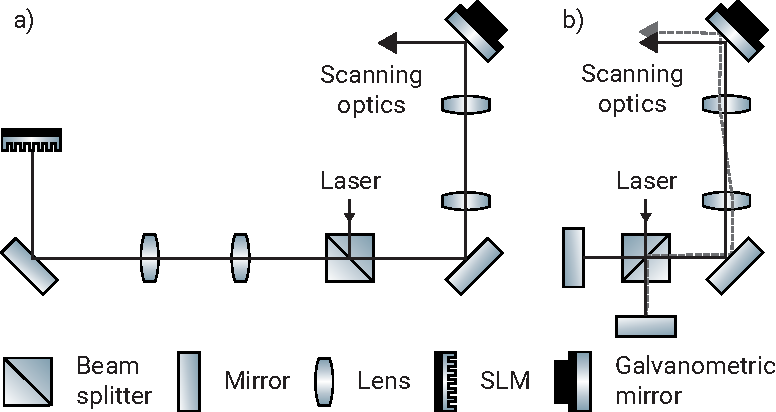
\includegraphics{dual_beam_layouts}
  \caption{Designs for each optical layout to create dual-beams in a light sheet system.
  a) Shows the conjugation of the SLM to the first scanning mirror, this technique suffered for optical losses on the SLM; discrete angular steps limited by the pixel size on the SLM and inhomogeneous distribution of power into each beam.
  b) Shows an optical solution for create two beams.
  }
  \label{fig:dual_beam_layouts}
\end{figure}

\subsubsection{Oversampling}
Conceivably, by driving the galvanometric mirrors at a very high frequency and pulsing a laser appropriately a sampling could be achieved that would appear to be two independent laser sources moving in unison.
This solution would require no additional optics.
The round trip time of the mirror, so that this sampling would be achieved, would in, the best case, would have to match the time it takes for the shutter to move up one row of pixels, $\frac{\SI{10}{\milli\second}}{1024}=\SI{9.8}{\micro\second}$.
The drive frequency would then exceed \SI{100}{\kilo\hertz}, which is currently infeasible with commercial scanning mirror technology and most affordable visible lasers.

\subsubsection{Optical approach}
An alternative method was employed whereby, immediately after all four colours were aligned spatially, a beam splitter was added with two returning mirrors, similar to Michelson interferometer.
Neither arm was interfered, instead they were purposely aimed off to create a small angle in their propagation before reaching the scanning mirror (Fig. \ref{fig:dual_beam_layouts} b).
This slight angular difference, once imaged through the telecentric scan lens, then became a spatial separation at the imaging plane of the system and was easily tuned using the kinematic mirrors flanking the beam splitter.

The all optical approach offered many advantages: the system was polarisation insensitive and suffered minimal optical losses, especially when compared to using an SLM.
As the duplication of the beams was now independent of any beam shaping, actual beam shaping optics could be readily implemented, this had the potential for optics such as cubic phase masks and axicon lenses or even an SLM being inserted to create the beam structure beams.

\begin{figure}
  \centering
  %\includegraphics[width=0.4\linewidth]{dualbeams/170517_40ms_exposure_488nm_58_amp_4_spacing}
  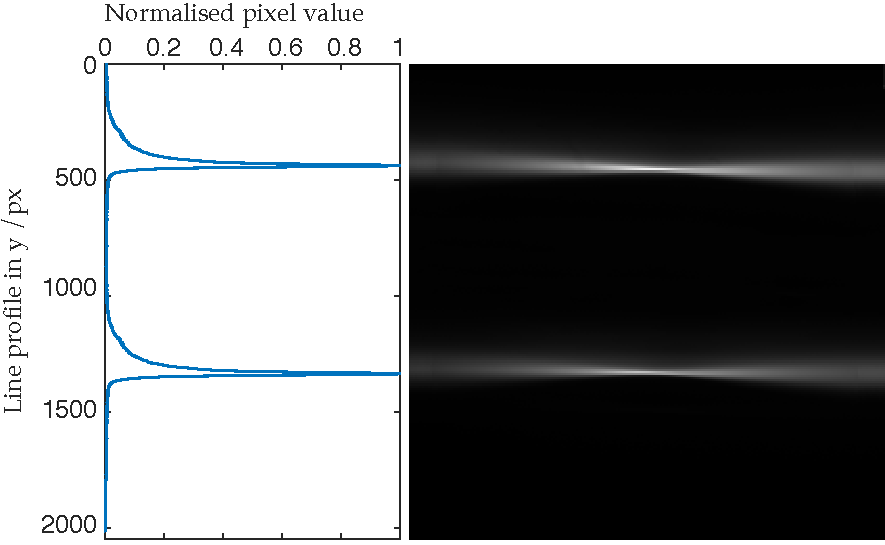
\includegraphics{dual_beam_profile}
  \caption{Fluoresence image of two beams at image plane as profiled by a solution of Rhodamine.}
  \label{fig:real_dual_beams}
\end{figure}

\subsubsection{Implementation}

Two laser beams were created at the image plane that could be manually separated (Fig. \ref{fig:real_dual_beams}).
To position the beams the correct distance apart, the bottom most beam was aligned to middle of the field of view by reducing the field of view the camera by half and digitally aligning the \emph{primary} beam with the bottom of the image using the galvanometric mirror.
The \emph{secondary} beam was pushed to the top of the image using the kinematic mirror below.

%\subsection{Implementation} % Talk about SLM options
%\subsubsection{Spatial light modulator} %Image of two beams with optimisation of intensity
%\subsubsection{All optical solution} %Polarisation insensitive better etc, option to make bessel.
 %\begin{figure}
%\centering
%\begin{subfigure}[b]{0.4\textwidth}
%  % This file was created by matlab2tikz.
%
%The latest updates can be retrieved from
%  http://www.mathworks.com/matlabcentral/fileexchange/22022-matlab2tikz-matlab2tikz
%where you can also make suggestions and rate matlab2tikz.
%
\definecolor{mycolor1}{rgb}{0.00000,0.44700,0.74100}%
%
\begin{tikzpicture}

\begin{axis}[%
width=0.984\figwidth,
height=\figheight,
at={(0\figwidth,0\figheight)},
scale only axis,
xmin=0,
xmax=25.5488,
xlabel style={font=\color{white!15!black}},
xlabel={Slit width ($\mu m$)},
ymin=0,
ymax=35,
ylabel style={font=\color{white!15!black}},
ylabel={Signal to noise (dB)},
axis background/.style={fill=white}
]
\addplot [color=red, line width=1.0pt, forget plot]
  table[row sep=crcr]{%
0	12.5324701883473\\
0.3576832	18.5517517631648\\
0.536524799999999	21.3039014622075\\
0.689817600000001	23.4232790372674\\
0.817561600000001	24.9922968789494\\
0.945305600000001	26.3719593165598\\
1.0475008	27.3391341147356\\
1.149696	28.1881179764521\\
1.2518912	28.9246702929426\\
1.3540864	29.5565914845402\\
1.4562816	30.0924366079897\\
1.5584768	30.5409615026896\\
1.660672	30.9107724682994\\
1.7373184	31.1415823689889\\
1.8139648	31.3363937054584\\
1.8906112	31.4986090923229\\
1.9672576	31.6314212951148\\
2.043904	31.7377184305017\\
2.1205504	31.8200496784818\\
2.1971968	31.8807095075506\\
2.2738432	31.921656218841\\
2.3504896	31.9444700886707\\
2.427136	31.9506564779818\\
2.5037824	31.9417335895084\\
2.5804288	31.9191863650125\\
2.682624	31.8704493184267\\
2.7848192	31.8032084295459\\
2.9125632	31.6973430270075\\
3.0403072	31.5715812950073\\
3.1936	31.4006216349322\\
3.3724416	31.1796939744442\\
3.6023808	30.8692886290347\\
4.3943936	29.7723786389734\\
4.6754304	29.4145838723353\\
4.9053696	29.1431481217906\\
5.10976	28.9229645190478\\
5.2886016	28.7507661513573\\
5.4674432	28.6000537380675\\
5.620736	28.4897926222317\\
5.7740288	28.3964151744919\\
5.9528704	28.3061194130879\\
6.131712	28.2322687465881\\
6.4127488	28.1341778614352\\
6.7959808	27.9996076335208\\
7.0770176	27.8818967737446\\
7.4857984	27.6922230883622\\
7.8179328	27.544064420835\\
8.0989696	27.4377257645978\\
8.4566528	27.3179030225738\\
8.686592	27.2550444145348\\
8.8909824	27.2141900807031\\
9.1464704	27.1802749839638\\
9.6318976	27.1219754606857\\
9.8107392	27.0837956630385\\
9.9384832	27.043406721796\\
10.0662272	26.9893810428362\\
10.1939712	26.9205807246331\\
10.3217152	26.8358290319353\\
10.4494592	26.7351311257944\\
10.602752	26.595798381566\\
10.7815936	26.4123055898538\\
11.3947648	25.7578797916527\\
11.5736064	25.6006521924437\\
11.7268992	25.4846361815047\\
11.9057408	25.370031240498\\
12.1101312	25.2583367066829\\
12.3400704	25.1497751558685\\
12.6977536	24.9841020246114\\
12.8765952	24.8819161534534\\
13.0554368	24.761050572625\\
13.3364736	24.5481946363449\\
13.6175104	24.3399978570067\\
13.8219008	24.2080664211949\\
14.0262912	24.094966399274\\
14.2051328	24.0111129567306\\
14.4095232	23.9325528641548\\
14.6394624	23.8600202360348\\
14.946048	23.7799278884203\\
15.2781824	23.6941292659659\\
15.5336704	23.609750113632\\
16.0701952	23.4111734157298\\
16.4278784	23.2662691793271\\
16.9388544	23.0497899994501\\
17.0921472	23.0019674102273\\
17.24544	22.9690905899991\\
17.4242816	22.9456730212193\\
17.756416	22.9070302681066\\
17.88416	22.8766954228097\\
18.011904	22.8299883099331\\
18.139648	22.7646530561944\\
18.267392	22.6801913558967\\
18.395136	22.5781940215279\\
18.5739776	22.4138293047022\\
19.0083072	22.0037067825766\\
19.2126976	21.8345218963388\\
19.4426368	21.6628033702563\\
19.672576	21.5088123471503\\
19.8769664	21.3886199511703\\
20.1069056	21.2707510455095\\
20.3879424	21.1464111214956\\
21.0522112	20.8695237016539\\
21.2821504	20.8003992970514\\
21.5376384	20.7392167038269\\
21.8186752	20.6873685361619\\
22.0486144	20.6585228243409\\
22.227456	20.6503914936922\\
22.3807488	20.6597387288038\\
22.5340416	20.6872139670611\\
22.7895296	20.7550469605905\\
23.0194688	20.8094057633795\\
23.2238592	20.8407290360167\\
23.4537984	20.8593348372081\\
23.6581888	20.8627008008416\\
23.8625792	20.8530215411433\\
24.0669696	20.828297025904\\
24.2969088	20.7840272342217\\
24.4757504	20.7358645169596\\
24.6290432	20.6821573848075\\
24.782336	20.6125987582598\\
24.9356288	20.5251825330413\\
25.1144704	20.4029380779673\\
25.3444096	20.2246438255472\\
25.5488	20.0579249772439\\
};
\addplot [color=mycolor1, line width=1.0pt, draw=none, mark size=0.3pt, mark=+, mark options={solid, mycolor1}, forget plot]
  table[row sep=crcr]{%
0	3.33157097627287\\
0.0512000000000015	5.68925090685172\\
0.102400000000003	10.9614618309317\\
0.153599999999997	14.4952519604569\\
0.204799999999999	15.5285276721776\\
0.256	17.392352214255\\
0.307200000000002	18.2809942304382\\
0.358400000000003	19.4791166036088\\
0.409599999999998	21.4462125283192\\
0.460799999999999	22.3779226769893\\
0.512	23.60526856644\\
0.563200000000002	23.8173634860006\\
0.614400000000003	24.1534082943417\\
0.665599999999998	24.7216382638042\\
0.716799999999999	25.9707033413741\\
0.768000000000001	26.9245821948088\\
0.819200000000002	26.2477625888218\\
0.870400000000004	27.2133481055704\\
0.921599999999998	27.4856058836931\\
0.972799999999999	27.7206312912012\\
1.024	28.0096287679877\\
1.0752	29.219584083895\\
1.1264	29.5542603822392\\
1.1776	28.7635548162973\\
1.2288	29.069052609128\\
1.28	29.6124691927918\\
1.3312	29.279061715928\\
1.3824	29.9655635733038\\
1.4336	29.8119346558916\\
1.4848	29.9961133070697\\
1.536	30.5849350438225\\
1.5872	30.4759179620393\\
1.6384	30.8477617633572\\
1.6896	30.8232050939703\\
1.7408	30.9801502573643\\
1.792	31.2361260039752\\
1.8432	30.7649743983784\\
1.8944	31.1424652129119\\
1.9456	31.1577464747291\\
1.9968	30.9449948522832\\
2.048	31.6485235890106\\
2.0992	31.3280642331209\\
2.1504	31.2421677788369\\
2.2016	31.1016289349603\\
2.2528	31.7583384570335\\
2.304	32.0933737896414\\
2.3552	31.9399800086695\\
2.4064	31.8884602887225\\
2.4576	31.8487761656517\\
2.5088	32.0705323540211\\
2.56	31.7337942238248\\
2.6112	31.5256627088902\\
2.6624	31.8330759337137\\
2.7136	31.870035713224\\
2.7648	31.346994756956\\
2.816	31.565557171603\\
2.8672	31.8868217178775\\
2.9184	31.7195245166921\\
2.9696	31.6320658688797\\
3.0208	31.3914276106829\\
3.072	31.0929416686075\\
3.1232	30.8140999017848\\
3.1744	31.3853596778172\\
3.2256	31.3865638218874\\
3.2768	31.0382759154048\\
3.328	31.1726766918085\\
3.3792	31.5471903527781\\
3.4304	31.4100656406078\\
3.4816	31.2781510084915\\
3.5328	31.275198308831\\
3.584	30.728584309306\\
3.6352	30.8695395280575\\
3.6864	30.8899049928459\\
3.7376	29.9708818761265\\
3.7888	30.5011385205577\\
3.84	30.2357903922359\\
3.8912	30.1647354305587\\
3.9424	30.2722270068091\\
3.9936	30.0158683315146\\
4.0448	30.2843546355019\\
4.096	30.4941285696048\\
4.1472	30.3984054677765\\
4.1984	29.7983423509278\\
4.2496	30.1136105396754\\
4.3008	29.384051483519\\
4.352	29.7875920088809\\
4.4032	30.1805692935572\\
4.4544	29.5799247132333\\
4.5056	29.340333077609\\
4.5568	30.195050351783\\
4.608	29.3025791472223\\
4.6592	29.2359266171225\\
4.7104	29.8260549304668\\
4.7616	28.8683927194053\\
4.8128	29.3703262754926\\
4.864	29.1437965194978\\
4.9152	29.6194810426113\\
4.9664	28.9098370458807\\
5.0176	28.9324122557613\\
5.0688	28.9672665773826\\
5.12	28.8913633640852\\
5.1712	28.5617937915253\\
5.2224	28.6151438666929\\
5.2736	28.9349491571461\\
5.3248	28.9617651765178\\
5.376	28.9723751251699\\
5.4272	28.5617511480488\\
5.4784	27.5555844801839\\
5.5296	28.3281852686811\\
5.5808	28.6917625827915\\
5.632	28.3785899516254\\
5.6832	28.1732279278933\\
5.7344	28.6667159072433\\
5.7856	28.0782517211234\\
5.8368	28.6512324839303\\
5.888	28.3680082810111\\
5.9392	27.9890840795493\\
5.9904	27.9690312276453\\
6.0416	28.0049465478969\\
6.0928	28.3401053577516\\
6.144	28.179335072071\\
6.1952	28.4754351125074\\
6.2464	27.9999423861978\\
6.2976	28.6024998441194\\
6.3488	28.7753664856823\\
6.4	27.6824480553023\\
6.4512	27.3254036045661\\
6.5024	28.1850127696641\\
6.5536	28.207507651015\\
6.6048	28.4166863755478\\
6.656	28.7726837304127\\
6.7072	28.3991668340173\\
6.7584	28.1720505747986\\
6.8096	27.6894478399653\\
6.8608	27.9073991434512\\
6.912	28.7879112664147\\
6.9632	27.6327554890617\\
7.0144	27.8117842842399\\
7.0656	27.5219413264581\\
7.1168	28.185703526591\\
7.168	27.5129307470291\\
7.2192	28.3233621373967\\
7.2704	27.9873929746941\\
7.3216	27.5288225874118\\
7.3728	28.1355250106854\\
7.424	27.6160012105201\\
7.4752	27.5872965670037\\
7.5264	28.0647048818702\\
7.5776	27.4161705267896\\
7.6288	27.4795774077182\\
7.68	27.6106077854599\\
7.7312	27.4318912666911\\
7.7824	26.9133754493193\\
7.8336	26.9917694271787\\
7.8848	27.4513682810223\\
7.936	27.3715200190877\\
7.9872	27.8654055151343\\
8.0384	27.5985824419912\\
8.0896	27.4407097442728\\
8.1408	27.7532807390385\\
8.192	27.8114636038919\\
8.2432	27.7729651485124\\
8.2944	27.0982414555755\\
8.3456	27.2058502802842\\
8.3968	27.5476587357558\\
8.448	27.0265435376141\\
8.4992	27.5556198185981\\
8.5504	27.3511544890779\\
8.6016	27.456674648579\\
8.6528	26.9144450127988\\
8.704	27.2991994100144\\
8.7552	26.3837990098108\\
8.8064	26.7901105274418\\
8.8576	27.2531838072191\\
8.9088	27.5115520835138\\
8.96	27.1207404881572\\
9.0112	26.9027476389701\\
9.0624	27.1647666588485\\
9.1136	27.0087446311655\\
9.1648	27.3189648586399\\
9.216	26.7387519690823\\
9.2672	27.8958503278519\\
9.3184	26.8493371112874\\
9.3696	27.4956272000903\\
9.4208	27.3138123628997\\
9.472	26.5341116515747\\
9.5232	26.5302340006265\\
9.5744	26.8035606563384\\
9.6256	27.4429575042321\\
9.6768	27.0563342672055\\
9.728	27.2307966451844\\
9.7792	27.3882405843507\\
9.8304	27.0022551068503\\
9.8816	27.4972657228721\\
9.9328	27.371928174205\\
9.984	27.5305993994251\\
10.0352	26.4148953021582\\
10.0864	27.0667696117873\\
10.1376	26.828624832721\\
10.1888	27.3131906276412\\
10.24	27.1968135773623\\
10.2912	27.4272694259507\\
10.3424	27.195639225009\\
10.3936	27.1649057447062\\
10.4448	26.4237252728889\\
10.496	26.4212207212489\\
10.5472	26.9697938620484\\
10.5984	26.7474523972065\\
10.6496	26.6843238335722\\
10.7008	26.7254857763761\\
10.752	27.275160320463\\
10.8032	26.0152841235038\\
10.8544	27.0922800013109\\
10.9056	26.4879682815236\\
10.9568	26.105905754072\\
11.008	25.7971081430827\\
11.0592	25.4975999415948\\
11.1104	25.5932353695968\\
11.1616	25.9408669378832\\
11.2128	25.5878996473285\\
11.264	25.7443682429912\\
11.3152	25.3277015661836\\
11.3664	26.0410107262767\\
11.4176	26.1322909897609\\
11.4688	25.0356254279006\\
11.52	25.7970960911737\\
11.5712	25.3379935864371\\
11.6224	25.4728134481539\\
11.6736	24.5407328441204\\
11.7248	25.1203156457113\\
11.776	25.4600907332422\\
11.8272	25.0245135799324\\
11.8784	25.3135250050148\\
11.9296	26.4458064179202\\
11.9808	25.5504236360066\\
12.032	25.0423623833142\\
12.0832	25.8298798245139\\
12.1344	24.1185731457101\\
12.1856	25.1812614581948\\
12.2368	25.3042920421267\\
12.288	24.8326515341304\\
12.3392	25.2958572654554\\
12.3904	24.4912378557932\\
12.4416	25.4498961560109\\
12.4928	24.3824949742688\\
12.544	25.0415252424034\\
12.5952	25.267789498229\\
12.6464	25.8948093296732\\
12.6976	25.3824141961407\\
12.7488	24.9217885826349\\
12.8	25.5079610499368\\
12.8512	25.6360320487683\\
12.9024	25.3031123110376\\
12.9536	24.6178233087841\\
13.0048	25.4993373841963\\
13.056	25.4242458376536\\
13.1072	24.596883427845\\
13.1584	24.2491394773646\\
13.2096	24.6898574669579\\
13.2608	24.6953107751152\\
13.312	24.7102781263956\\
13.3632	24.4434875195332\\
13.4144	24.2564362429528\\
13.4656	24.2739966764863\\
13.5168	24.5187834865567\\
13.568	23.6497686962786\\
13.6192	23.7671738118711\\
13.6704	24.1699025714421\\
13.7216	24.2734539675945\\
13.7728	24.2014921542657\\
13.824	24.0471438158033\\
13.8752	24.27377881661\\
13.9264	24.0803399780494\\
13.9776	24.2937929988754\\
14.0288	24.2510149114913\\
14.08	24.4122639585329\\
14.1312	23.6271430013138\\
14.1824	23.9172639551884\\
14.2336	22.784547617336\\
14.2848	24.2567448266865\\
14.336	24.3638915940614\\
14.3872	24.0920710784737\\
14.4384	23.3973364842536\\
14.4896	24.3372738730219\\
14.5408	24.2761846528712\\
14.592	23.9299577996235\\
14.6432	23.169825161711\\
14.6944	24.0490859885747\\
14.7456	23.5907286260664\\
14.7968	24.3884069829063\\
14.848	24.2820989316269\\
14.8992	22.8636400485754\\
14.9504	22.2469189978662\\
15.0016	23.8670999735808\\
15.0528	23.8294984065328\\
15.104	24.9845504533986\\
15.1552	23.9218986749876\\
15.2064	24.3259663360374\\
15.2576	23.9180430731922\\
15.3088	23.4612903968186\\
15.36	24.4695540635553\\
15.4112	23.7874501532374\\
15.4624	23.6241761467617\\
15.5136	23.8971140026301\\
15.5648	22.7066896407471\\
15.616	23.3706351048901\\
15.6672	23.4730673406815\\
15.7184	23.1465707471484\\
15.7696	23.7101878190538\\
15.8208	23.5997888415707\\
15.872	23.5676095155672\\
15.9232	23.7999241445799\\
15.9744	23.517343128102\\
16.0256	22.6264923639352\\
16.0768	23.0833732858098\\
16.128	23.7103802499292\\
16.1792	22.8035798641189\\
16.2304	23.7413819574107\\
16.2816	23.5927287180809\\
16.3328	23.9687952713252\\
16.384	23.7233537090989\\
16.4352	23.419351565343\\
16.4864	23.1275607120496\\
16.5376	23.7310521534922\\
16.5888	23.0158307641527\\
16.64	23.1540507447235\\
16.6912	23.2529084126749\\
16.7424	23.1610940608131\\
16.7936	23.1271163848495\\
16.8448	23.613575047698\\
16.896	22.980307523891\\
16.9472	23.2333951019559\\
16.9984	21.8399473947643\\
17.0496	22.1342392736309\\
17.1008	22.1287437204873\\
17.152	23.1252494353267\\
17.2032	22.7673568769466\\
17.2544	22.6390189704222\\
17.3056	22.9760972746216\\
17.3568	21.9707918293806\\
17.408	22.7576612689441\\
17.4592	22.6046426835303\\
17.5104	23.2396048016377\\
17.5616	22.338713540093\\
17.6128	22.8541903864319\\
17.664	23.7569377776128\\
17.7152	22.6106403614906\\
17.7664	23.5010971640545\\
17.8176	22.4237026236807\\
17.8688	23.3539109714287\\
17.92	24.4830204474958\\
17.9712	22.99970728599\\
18.0224	22.3692180236815\\
18.0736	23.3764623875242\\
18.1248	23.5118868208358\\
18.176	22.9700866848743\\
18.2272	23.0430563255527\\
18.2784	23.1749834949706\\
18.3296	23.1677184363428\\
18.3808	22.9788722115412\\
18.432	23.4235819780562\\
18.4832	22.4216810385032\\
18.5344	22.6458819259142\\
18.5856	21.6622957584951\\
18.6368	22.3071734678409\\
18.688	22.2050907833038\\
18.7392	21.7252792952781\\
18.7904	21.2558372266239\\
18.8416	22.1536849340094\\
18.8928	21.348137828446\\
18.944	22.4698575121449\\
18.9952	21.4354539281262\\
19.0464	21.3369852508053\\
19.0976	21.6288797227948\\
19.1488	21.8232004957545\\
19.2	22.2571474752984\\
19.2512	21.7196574200843\\
19.3024	22.2612431257671\\
19.3536	22.2073649196449\\
19.4048	20.7575397493212\\
19.456	22.1404219927528\\
19.5072	21.1690682191128\\
19.5584	22.5591377361857\\
19.6096	22.1596346730768\\
19.6608	20.6336434261345\\
19.712	20.5957571010323\\
19.7632	21.396542282208\\
19.8144	21.4384805313111\\
19.8656	21.9953564140802\\
19.9168	21.4100515063561\\
19.968	21.2800520305288\\
20.0192	21.5159591147211\\
20.0704	20.2103491371968\\
20.1216	21.5790150376316\\
20.1728	21.4893283384523\\
20.224	19.6746883653391\\
20.2752	21.071600335482\\
20.3264	21.8294625651202\\
20.3776	21.693723443709\\
20.4288	21.4948775880129\\
20.48	21.6438774536702\\
20.5312	21.1330638179253\\
20.5824	21.9853462620584\\
20.6336	21.2978316813053\\
20.6848	21.2749012213742\\
20.736	21.3773189685659\\
20.7872	20.0520453022057\\
20.8384	20.8526383236591\\
20.8896	20.755737352493\\
20.9408	20.7270743859019\\
20.992	19.4665181448848\\
21.0432	21.2459157536449\\
21.0944	20.9208826698866\\
21.1456	20.5376373222831\\
21.1968	21.3934904529709\\
21.248	20.073935294696\\
21.2992	21.2572843587237\\
21.3504	20.8772635965902\\
21.4016	21.2328148002806\\
21.4528	20.4864587321981\\
21.504	20.9685323029608\\
21.5552	20.4751812021882\\
21.6064	20.9976246972374\\
21.6576	20.3139657301293\\
21.7088	21.1601748504969\\
21.76	20.9379010675784\\
21.8112	20.5701403958066\\
21.8624	21.0258471369656\\
21.9136	20.3643351999575\\
21.9648	21.6654154307242\\
22.016	20.7133548778145\\
22.0672	20.7623390187802\\
22.1184	20.3310088300586\\
22.1696	20.925617423939\\
22.2208	20.9789032772669\\
22.272	19.9650405588763\\
22.3232	20.275412508617\\
22.3744	19.2623467327039\\
22.4256	19.5525442268124\\
22.4768	19.5574787764008\\
22.528	20.733287071133\\
22.5792	20.5108858200885\\
22.6304	20.9137488171879\\
22.6816	20.8551593999367\\
22.7328	21.0608053301758\\
22.784	21.2087511540249\\
22.8352	21.3139975062827\\
22.8864	21.4216633061901\\
22.9376	21.0346880859577\\
22.9888	21.2404518477675\\
23.04	21.3009578153953\\
23.0912	20.303782214726\\
23.1424	21.6087107284691\\
23.1936	20.954323929056\\
23.2448	20.7881756003123\\
23.296	20.3461138563686\\
23.3472	20.6505913604183\\
23.3984	20.3348558106543\\
23.4496	20.903574195678\\
23.5008	21.250547450692\\
23.552	21.2020788001322\\
23.6032	21.0629089717655\\
23.6544	19.9054795125792\\
23.7056	20.87409156142\\
23.7568	21.0432484980418\\
23.808	20.8848116402958\\
23.8592	20.5869466457439\\
23.9104	21.2977800316899\\
23.9616	21.5958506948603\\
24.0128	21.2671542722022\\
24.064	20.0592416247566\\
24.1152	20.2113433000149\\
24.1664	20.0331393246308\\
24.2176	21.1765845515351\\
24.2688	21.1960198526055\\
24.32	21.0040203940998\\
24.3712	19.892806348358\\
24.4224	21.0871898033115\\
24.4736	20.2957274313882\\
24.5248	20.0792711697381\\
24.576	20.9237916960231\\
24.6272	21.0351180484178\\
24.6784	21.5297196162854\\
24.7296	20.6168624941274\\
24.7808	20.6714906131625\\
24.832	21.4125163758362\\
24.8832	20.8375998365272\\
24.9344	20.4728521952436\\
24.9856	20.8846357827997\\
25.0368	20.880005679696\\
25.088	19.8136333829317\\
25.1392	20.8536651120271\\
25.1904	20.2482601628627\\
25.2416	20.5831256984835\\
25.2928	19.2603033464767\\
25.344	20.1336842485657\\
25.3952	20.9359074727279\\
25.4464	20.1950481628567\\
25.4976	18.5356867461123\\
25.5488	20.190291026928\\
};
\end{axis}
\end{tikzpicture}%
%  \caption{You a beaut}
%  \end{subfigure}%
%\begin{subfigure}[b]{0.4\textwidth}
%    \centering
%  % This file was created by matlab2tikz.
%
%The latest updates can be retrieved from
%  http://www.mathworks.com/matlabcentral/fileexchange/22022-matlab2tikz-matlab2tikz
%where you can also make suggestions and rate matlab2tikz.
%
\definecolor{mycolor1}{rgb}{0.00000,0.44700,0.74100}%
%
\begin{tikzpicture}

\begin{axis}[%
width=0.984\figwidth,
height=\figheight,
at={(0\figwidth,0\figheight)},
scale only axis,
xmin=0,
xmax=25.5488,
xlabel style={font=\color{white!15!black}},
xlabel={Slit width ($\mu m$)},
ymin=0,
ymax=1,
ylabel style={font=\color{white!15!black}},
ylabel={Contrast ($A.U$)},
axis background/.style={fill=white}
]
\addplot [color=red, line width=1.0pt, forget plot]
  table[row sep=crcr]{%
0	0.053533133170852\\
0.281036799999999	0.213402741295727\\
0.408780799999999	0.285206170000027\\
0.510975999999999	0.341732206661433\\
0.587622400000001	0.383364871289366\\
0.664268799999999	0.424186474573705\\
0.7409152	0.464051585760803\\
0.817561600000001	0.502811584132566\\
0.8686592	0.527971352337268\\
0.919756800000002	0.552542968494336\\
0.9708544	0.576489511077249\\
1.021952	0.599774626968589\\
1.0730496	0.62236389996632\\
1.1241472	0.644226847903152\\
1.1752448	0.665341206050776\\
1.2263424	0.685693927814473\\
1.27744	0.705273886222056\\
1.3285376	0.724069940188681\\
1.3796352	0.742073887786162\\
1.4307328	0.759278981570493\\
1.4818304	0.775681414282769\\
1.532928	0.791277589021568\\
1.5840256	0.806065209876682\\
1.6351232	0.820045859456719\\
1.6862208	0.833221828295489\\
1.7373184	0.845599175525479\\
1.788416	0.857187074452838\\
1.8395136	0.867995669321441\\
1.8906112	0.878036951635842\\
1.9417088	0.887321664883331\\
1.9928064	0.895858812323372\\
2.043904	0.903656046400027\\
2.0950016	0.910720291915315\\
2.1460992	0.917060649154546\\
2.1971968	0.92268535785329\\
2.2482944	0.927600124597948\\
2.299392	0.931807733723748\\
2.3504896	0.935313349188931\\
2.4015872	0.938127644471308\\
2.4526848	0.940265473586123\\
2.5037824	0.941746323085091\\
2.55488	0.942593642270474\\
2.6059776	0.942836700925788\\
2.6570752	0.942506908494114\\
2.7081728	0.941634963752481\\
2.7848192	0.939379290968024\\
2.8614656	0.936082109939886\\
2.938112	0.93183937206577\\
3.0147584	0.926753307616828\\
3.0914048	0.92092658171352\\
3.1680512	0.914449006721803\\
3.2702464	0.904904927548014\\
3.3724416	0.894419642547284\\
3.4746368	0.883095654290056\\
3.6023808	0.867990431477718\\
3.7556736	0.848978947034574\\
4.215552	0.791422747701883\\
4.3943936	0.769828571349098\\
4.5732352	0.749061574413609\\
4.726528	0.732081440775975\\
4.854272	0.718695711155405\\
4.982016	0.706181556976002\\
5.0842112	0.696913916435172\\
5.1864064	0.688374614855434\\
5.2886016	0.680591788641596\\
5.3907968	0.673551954991346\\
5.492992	0.667251380162465\\
5.5951872	0.661692394749057\\
5.6973824	0.656829291999227\\
5.7995776	0.652614797448958\\
5.9273216	0.648172944482084\\
6.0550656	0.644523964289082\\
6.2339072	0.64032401328053\\
6.6682368	0.630661630743187\\
6.8470784	0.625644854034103\\
7.0770176	0.618311591622057\\
7.7157376	0.597350310841119\\
7.8945792	0.592485016491658\\
8.1245184	0.587014200485463\\
8.4055552	0.581018019407502\\
8.6354944	0.576806943406513\\
8.8398848	0.573823942729785\\
9.069824	0.571378520281115\\
9.6829952	0.565737479590279\\
9.836288	0.563320283656726\\
9.964032	0.560567675856511\\
10.091776	0.556994004900123\\
10.21952	0.552526578615613\\
10.3217152	0.548255557772034\\
10.4494592	0.542064753585823\\
10.5772032	0.535045714537418\\
10.730496	0.525730822416936\\
10.9093376	0.514002886760288\\
11.2159232	0.493810781751495\\
11.369216	0.484581188840597\\
11.49696	0.477582513348597\\
11.624704	0.471321047958014\\
11.752448	0.465852624707018\\
11.880192	0.461127230192947\\
12.0334848	0.456230074060688\\
12.2123264	0.451344420537275\\
12.4167168	0.446586956307197\\
12.7999488	0.437979457098564\\
12.9787904	0.43307500732098\\
13.1831808	0.426632453476532\\
13.796352	0.406599605449383\\
14.0007424	0.40104632929269\\
14.2051328	0.396192796634903\\
14.4606208	0.391007022099018\\
14.7416576	0.386044399752542\\
15.073792	0.381030376947702\\
15.3548288	0.376573561092219\\
16.1723904	0.362690362623827\\
16.5300736	0.356757624475325\\
16.9133056	0.350273074095195\\
17.0665984	0.348450081027078\\
17.2198912	0.347378753501634\\
17.3987328	0.346924852322203\\
17.756416	0.346362494221715\\
17.88416	0.345406005581641\\
18.011904	0.343699543376321\\
18.139648	0.341160723479202\\
18.267392	0.337763064933032\\
18.395136	0.333577629249305\\
18.5739776	0.326787260016243\\
18.9572096	0.311856199143108\\
19.1616	0.3048514945602\\
19.3659904	0.298639651264036\\
19.5703808	0.293222483023399\\
19.7747712	0.288572159739459\\
20.0302592	0.283617316402136\\
20.6434304	0.272234344163056\\
21.0266624	0.264615955368281\\
21.2310528	0.261295398935562\\
21.4098944	0.259100049312806\\
21.588736	0.257733685074257\\
21.7675776	0.257164992376911\\
21.9464192	0.257315574164767\\
22.1508096	0.258279853056514\\
22.3296512	0.259878986296766\\
22.5084928	0.26227884852953\\
23.0705664	0.270689648845003\\
23.249408	0.272249499133807\\
23.4537984	0.27323757821463\\
23.6581888	0.273469757339225\\
23.8625792	0.272985100890768\\
24.0669696	0.271765063657345\\
24.3224576	0.269417183176628\\
24.6034944	0.265998640471505\\
24.8589824	0.262111818131405\\
25.0633728	0.25828909634884\\
25.3444096	0.25215246590389\\
25.5488	0.247452511028669\\
};
\addplot [color=mycolor1, line width=1.0pt, draw=none, mark size=0.3pt, mark=+, mark options={solid, mycolor1}, forget plot]
  table[row sep=crcr]{%
0	0\\
0.0512000000000015	0.0280886215929712\\
0.102399999999999	0.0708206343359237\\
0.153600000000001	0.111735187820759\\
0.204799999999999	0.129103459291429\\
0.256	0.164498281909548\\
0.307200000000002	0.193988570483892\\
0.3584	0.218630921952538\\
0.409600000000001	0.284635554714473\\
0.460799999999999	0.314513668740915\\
0.512	0.354365873710641\\
0.563199999999998	0.380793466913467\\
0.6144	0.373057608022531\\
0.665600000000001	0.408459972441246\\
0.716799999999999	0.482908739779301\\
0.768000000000001	0.511274957722836\\
0.819199999999999	0.50098880849707\\
0.8704	0.537583568778306\\
0.921600000000002	0.55378965249378\\
0.972799999999999	0.593553735647088\\
1.024	0.625759939954975\\
1.0752	0.690212811080769\\
1.1264	0.730354679838086\\
1.1776	0.66526876263487\\
1.2288	0.679117762905211\\
1.28	0.741905940191074\\
1.3312	0.723492042197858\\
1.3824	0.778760676332723\\
1.4336	0.750327598399277\\
1.4848	0.785008952295346\\
1.536	0.83641535865095\\
1.5872	0.793032642933323\\
1.6384	0.86308753938053\\
1.6896	0.856734002121566\\
1.7408	0.845403326475004\\
1.792	0.883125676396627\\
1.8432	0.849210949041954\\
1.8944	0.866945655367005\\
1.9456	0.878640255728765\\
1.9968	0.884989580886121\\
2.048	0.935783216656851\\
2.0992	0.894804419127645\\
2.1504	0.900434991231567\\
2.2016	0.889981053662343\\
2.2528	0.956466513694881\\
2.304	0.981058182278481\\
2.3552	0.959464237820264\\
2.4064	0.979366552059364\\
2.4576	0.961203123822969\\
2.5088	1\\
2.56	0.949611506167329\\
2.6112	0.931706892899005\\
2.6624	0.946002893087691\\
2.7136	0.969525144829078\\
2.7648	0.899700855402415\\
2.816	0.915545038564741\\
2.8672	0.972469151144779\\
2.9184	0.940729552741647\\
2.9696	0.912733539633724\\
3.0208	0.912062076399067\\
3.072	0.890361087158418\\
3.1232	0.850862808558201\\
3.1744	0.898792983600888\\
3.2256	0.912817520031883\\
3.2768	0.899103794312246\\
3.328	0.890295447115406\\
3.3792	0.937903738848167\\
3.4304	0.921676679997137\\
3.4816	0.904345418121601\\
3.5328	0.891272187195316\\
3.584	0.851212320239743\\
3.6352	0.875909140598683\\
3.6864	0.891463779045822\\
3.7376	0.781310246287436\\
3.7888	0.820803043798865\\
3.84	0.813459719339853\\
3.8912	0.792901541627721\\
3.9424	0.784867742476429\\
3.9936	0.806288134122639\\
4.0448	0.805475427214979\\
4.096	0.848771874861036\\
4.1472	0.824082608631361\\
4.1984	0.788720920896669\\
4.2496	0.780184433766898\\
4.3008	0.747731607700089\\
4.352	0.757182929465444\\
4.4032	0.788518901115104\\
4.4544	0.771499074157841\\
4.5056	0.737528947929345\\
4.5568	0.808881672255541\\
4.608	0.744364631149175\\
4.6592	0.716562788653487\\
4.7104	0.783425503092431\\
4.7616	0.693107390561774\\
4.8128	0.734733343196375\\
4.864	0.707921219998731\\
4.9152	0.756214587767115\\
4.9664	0.654291848556028\\
5.0176	0.687209051376499\\
5.0688	0.697841662446486\\
5.12	0.677774671841686\\
5.1712	0.658562528448236\\
5.2224	0.656454662432985\\
5.2736	0.694265604985382\\
5.3248	0.691679112092316\\
5.376	0.706620617497197\\
5.4272	0.667249856995127\\
5.4784	0.591697244713586\\
5.5296	0.657109056022801\\
5.5808	0.693676018365213\\
5.632	0.6468466383619\\
5.6832	0.641504227363392\\
5.7344	0.670305703013554\\
5.7856	0.632551733904407\\
5.8368	0.664907498310502\\
5.888	0.628249451431238\\
5.9392	0.631014161961183\\
5.9904	0.619435288999583\\
6.0416	0.616060297021733\\
6.0928	0.656916202722982\\
6.144	0.638685602900583\\
6.1952	0.652652118228154\\
6.2464	0.649075546045452\\
6.2976	0.653734516848452\\
6.3488	0.681486024052397\\
6.4	0.612000007289936\\
6.4512	0.590418315798615\\
6.5024	0.629945244632669\\
6.5536	0.677373920759067\\
6.6048	0.667652117850583\\
6.656	0.696231449317327\\
6.7072	0.664757719664081\\
6.7584	0.637432040759727\\
6.8096	0.611484048552924\\
6.8608	0.624211342694895\\
6.912	0.660589166784771\\
6.9632	0.607968354850861\\
7.0144	0.603315333201628\\
7.0656	0.588783756038893\\
7.1168	0.637655021366552\\
7.168	0.593272170552648\\
7.2192	0.638318054613734\\
7.2704	0.617585184980214\\
7.3216	0.623883481310983\\
7.3728	0.625999743384586\\
7.424	0.586648117072158\\
7.4752	0.589096869447687\\
7.5264	0.613639702850627\\
7.5776	0.589252355897798\\
7.6288	0.588217236333776\\
7.68	0.598241118777832\\
7.7312	0.592963243340737\\
7.7824	0.540685098285309\\
7.8336	0.56770081691004\\
7.8848	0.599451950151991\\
7.936	0.580477217869994\\
7.9872	0.612244984465899\\
8.0384	0.599155444687586\\
8.0896	0.59481389394109\\
8.1408	0.598060734626486\\
8.192	0.606118370326843\\
8.2432	0.619035257920672\\
8.2944	0.55912359253108\\
8.3456	0.571790221992288\\
8.3968	0.592660166862572\\
8.448	0.548580165627776\\
8.4992	0.606048463316853\\
8.5504	0.591306913755751\\
8.6016	0.60975761711892\\
8.6528	0.544554616143824\\
8.704	0.578013600813115\\
8.7552	0.505426284640521\\
8.8064	0.559368950981785\\
8.8576	0.589728039665761\\
8.9088	0.604153892767879\\
8.96	0.576170538963076\\
9.0112	0.527873094052321\\
9.0624	0.54933330434773\\
9.1136	0.545247491061172\\
9.1648	0.598756353275824\\
9.216	0.540847853247094\\
9.2672	0.616195183677064\\
9.3184	0.565473759232095\\
9.3696	0.582639292603275\\
9.4208	0.580999866325818\\
9.472	0.544841076294002\\
9.5232	0.535911986203974\\
9.5744	0.529896964377336\\
9.6256	0.59284841604169\\
9.6768	0.561133519816554\\
9.728	0.579284342810201\\
9.7792	0.556510606889518\\
9.8304	0.555331963246779\\
9.8816	0.586170941171826\\
9.9328	0.594826678413487\\
9.984	0.606643918317044\\
10.0352	0.493844883047647\\
10.0864	0.566735262399099\\
10.1376	0.549404295700334\\
10.1888	0.594312114555596\\
10.24	0.572338767977755\\
10.2912	0.577940686197891\\
10.3424	0.568027028974306\\
10.3936	0.573385334677813\\
10.4448	0.523596005895655\\
10.496	0.539866463996454\\
10.5472	0.539308889734606\\
10.5984	0.526095832282536\\
10.6496	0.541247492579231\\
10.7008	0.544198640553127\\
10.752	0.576580951573654\\
10.8032	0.501592413928616\\
10.8544	0.552463513941017\\
10.9056	0.508186440265984\\
10.9568	0.506285916957147\\
11.008	0.501596759368855\\
11.0592	0.482368258338433\\
11.1104	0.478438117703728\\
11.1616	0.492714957052989\\
11.2128	0.469251523200558\\
11.264	0.484536517901347\\
11.3152	0.465777861095301\\
11.3664	0.492523033181847\\
11.4176	0.502531188151952\\
11.4688	0.445171980196086\\
11.52	0.483145614380749\\
11.5712	0.451654552146664\\
11.6224	0.458342787322088\\
11.6736	0.429640282362442\\
11.7248	0.445028608678872\\
11.776	0.448201524663379\\
11.8272	0.456590262437484\\
11.8784	0.444403101157565\\
11.9296	0.507421495047247\\
11.9808	0.483161055618549\\
12.032	0.442676119825443\\
12.0832	0.483817086486781\\
12.1344	0.406257625271135\\
12.1856	0.458027881784769\\
12.2368	0.457690866983814\\
12.288	0.428950115417809\\
12.3392	0.446725229283555\\
12.3904	0.41831184530394\\
12.4416	0.446395723501592\\
12.4928	0.430354071463182\\
12.544	0.43549909704922\\
12.5952	0.446642085654119\\
12.6464	0.488746237246509\\
12.6976	0.462523576966891\\
12.7488	0.433599821187734\\
12.8	0.460680741840015\\
12.8512	0.468837001290574\\
12.9024	0.45068411307907\\
12.9536	0.425508202436152\\
13.0048	0.47007679838244\\
13.056	0.448215274623418\\
13.1072	0.4140182723621\\
13.1584	0.419734370701921\\
13.2096	0.444778394816442\\
13.2608	0.436337837829843\\
13.312	0.433001929076276\\
13.3632	0.406017495006402\\
13.4144	0.410180484359518\\
13.4656	0.412638606427066\\
13.5168	0.419243865643054\\
13.568	0.386705483106113\\
13.6192	0.390914709580617\\
13.6704	0.393174318633537\\
13.7216	0.413585874208852\\
13.7728	0.391890562595894\\
13.824	0.399942051306457\\
13.8752	0.430883282843649\\
13.9264	0.394391301366813\\
13.9776	0.409616770271349\\
14.0288	0.401217354748681\\
14.08	0.40371780392794\\
14.1312	0.369844717281371\\
14.1824	0.38700956382964\\
14.2336	0.354240258136628\\
14.2848	0.405198831006739\\
14.336	0.433009546794182\\
14.3872	0.408314368347078\\
14.4384	0.379495964794241\\
14.4896	0.41145037524927\\
14.5408	0.395189587774471\\
14.592	0.380472770493025\\
14.6432	0.358507107130134\\
14.6944	0.401076330591856\\
14.7456	0.365150801199192\\
14.7968	0.413482678275447\\
14.848	0.390379356261025\\
14.8992	0.338540179370014\\
14.9504	0.335043466506502\\
15.0016	0.387238325402258\\
15.0528	0.367093485474175\\
15.104	0.433543094888662\\
15.1552	0.376868577685403\\
15.2064	0.427370407058078\\
15.2576	0.409367319343225\\
15.3088	0.374853047384438\\
15.36	0.391801736904505\\
15.4112	0.37706565838371\\
15.4624	0.370851269188247\\
15.5136	0.379964842309352\\
15.5648	0.36300856757385\\
15.616	0.364678964240522\\
15.6672	0.356971307104654\\
15.7184	0.349951041470799\\
15.7696	0.361923605868434\\
15.8208	0.364499182527709\\
15.872	0.369081790697013\\
15.9232	0.362716910513743\\
15.9744	0.381112660435303\\
16.0256	0.332583939804742\\
16.0768	0.342184849898246\\
16.128	0.395436649924171\\
16.1792	0.346949521988876\\
16.2304	0.346730565537349\\
16.2816	0.376622808190366\\
16.3328	0.375053885518408\\
16.384	0.387402353227117\\
16.4352	0.38486698169076\\
16.4864	0.368915784045225\\
16.5376	0.389887861205995\\
16.5888	0.353892399528757\\
16.64	0.344574609456103\\
16.6912	0.355111932062929\\
16.7424	0.372019789823572\\
16.7936	0.350953638654858\\
16.8448	0.367669539275013\\
16.896	0.311069198599231\\
16.9472	0.365247519200938\\
16.9984	0.30433624062098\\
17.0496	0.314994862419436\\
17.1008	0.307167797540767\\
17.152	0.345438936498557\\
17.2032	0.336146614919951\\
17.2544	0.327501886523354\\
17.3056	0.324222606375066\\
17.3568	0.31417887759229\\
17.408	0.340029049070406\\
17.4592	0.352677286677675\\
17.5104	0.37513032146126\\
17.5616	0.315929075638238\\
17.6128	0.339643140284601\\
17.664	0.356637700595218\\
17.7152	0.354462716774474\\
17.7664	0.375219713655749\\
17.8176	0.342288874690144\\
17.8688	0.376724679981759\\
17.92	0.39735202953452\\
17.9712	0.338708123963563\\
18.0224	0.332616537594486\\
18.0736	0.352395242717282\\
18.1248	0.389603082091945\\
18.176	0.344876806540768\\
18.2272	0.354165230538175\\
18.2784	0.370408955053456\\
18.3296	0.368839998600631\\
18.3808	0.346977666383129\\
18.432	0.36970483596156\\
18.4832	0.322178212835098\\
18.5344	0.318023827816702\\
18.5856	0.306761365377106\\
18.6368	0.311435665092691\\
18.688	0.329224433880295\\
18.7392	0.288518738898443\\
18.7904	0.269678722793554\\
18.8416	0.320519564446414\\
18.8928	0.289750126043835\\
18.944	0.311805223322853\\
18.9952	0.302602007870728\\
19.0464	0.287551845797804\\
19.0976	0.303585017736701\\
19.1488	0.299745142689908\\
19.2	0.321451981577596\\
19.2512	0.311304774458453\\
19.3024	0.313728920697361\\
19.3536	0.297228470193474\\
19.4048	0.253888001437179\\
19.456	0.319874782642231\\
19.5072	0.270835524358095\\
19.5584	0.327417639980652\\
19.6096	0.301587426435031\\
19.6608	0.246507442738679\\
19.712	0.277257338547525\\
19.7632	0.289109193893232\\
19.8144	0.297775276993818\\
19.8656	0.298627825379413\\
19.9168	0.282212741374785\\
19.968	0.262745323669964\\
20.0192	0.288293771582428\\
20.0704	0.253285911556528\\
20.1216	0.318732522573761\\
20.1728	0.288316637391397\\
20.224	0.237221469387539\\
20.2752	0.274916581476628\\
20.3264	0.300146321053735\\
20.3776	0.303854041055615\\
20.4288	0.304214932321948\\
20.48	0.301307423440953\\
20.5312	0.284544348563159\\
20.5824	0.29797172957899\\
20.6336	0.278428304564802\\
20.6848	0.268602600222444\\
20.736	0.259432599347946\\
20.7872	0.251181059143494\\
20.8384	0.268295278141107\\
20.8896	0.266864539258552\\
20.9408	0.276534509315582\\
20.992	0.225709619056669\\
21.0432	0.272178900425349\\
21.0944	0.272182537834087\\
21.1456	0.275048195211113\\
21.1968	0.281937444866426\\
21.248	0.238122016048589\\
21.2992	0.245818174137863\\
21.3504	0.259655595825631\\
21.4016	0.25650500162272\\
21.4528	0.232013587050737\\
21.504	0.234865210127911\\
21.5552	0.276617799706944\\
21.6064	0.256895856773038\\
21.6576	0.257826163628184\\
21.7088	0.258974076650322\\
21.76	0.260309546638233\\
21.8112	0.247165091090999\\
21.8624	0.259375353547522\\
21.9136	0.251549772234281\\
21.9648	0.281385392349886\\
22.016	0.273756614696818\\
22.0672	0.257338577770334\\
22.1184	0.26053597041302\\
22.1696	0.275315664532364\\
22.2208	0.244272718060611\\
22.272	0.251108078050827\\
22.3232	0.2485842809925\\
22.3744	0.211005340963197\\
22.4256	0.235770394366796\\
22.4768	0.219328507862983\\
22.528	0.271301941383232\\
22.5792	0.265956668321845\\
22.6304	0.271304754525335\\
22.6816	0.268034814320721\\
22.7328	0.258245562196624\\
22.784	0.280078704877511\\
22.8352	0.294203526869737\\
22.8864	0.305002787113988\\
22.9376	0.253759695364458\\
22.9888	0.287317625015934\\
23.04	0.306228109121076\\
23.0912	0.256394905421644\\
23.1424	0.290216344672871\\
23.1936	0.257687717874934\\
23.2448	0.288534837555538\\
23.296	0.26641527466904\\
23.3472	0.280668515654632\\
23.3984	0.245714157273131\\
23.4496	0.281555376201599\\
23.5008	0.270533393599997\\
23.552	0.283513777873377\\
23.6032	0.275815011856317\\
23.6544	0.254825936489471\\
23.7056	0.272576690566698\\
23.7568	0.268931826694832\\
23.808	0.276046375353527\\
23.8592	0.279224814737091\\
23.9104	0.283480762076376\\
23.9616	0.297230718214525\\
24.0128	0.28181396998777\\
24.064	0.255243336799857\\
24.1152	0.253559280953077\\
24.1664	0.259723280444391\\
24.2176	0.283910554713128\\
24.2688	0.262581064410508\\
24.32	0.275299651294084\\
24.3712	0.259561656773307\\
24.4224	0.283832379149491\\
24.4736	0.246116911513525\\
24.5248	0.260796056045837\\
24.576	0.260987423323282\\
24.6272	0.272016396637685\\
24.6784	0.2668158009972\\
24.7296	0.24240095124032\\
24.7808	0.262223165192786\\
24.832	0.278062920056037\\
24.8832	0.27549169824713\\
24.9344	0.26672215946958\\
24.9856	0.287658175663207\\
25.0368	0.261444361245768\\
25.088	0.24565518411222\\
25.1392	0.28253004544867\\
25.1904	0.253339091642523\\
25.2416	0.264347569548288\\
25.2928	0.224205937278764\\
25.344	0.235658121722029\\
25.3952	0.27515952742851\\
25.4464	0.24520713251087\\
25.4976	0.209538974472625\\
25.5488	0.257418386881323\\
};
\end{axis}
\end{tikzpicture}%
%  \caption{You a beaut}
%  \end{subfigure}%
%\end{figure}

\section{Structured illumination}

%Confocal slit scanning extends the pass band of the objective to up double in one direction.
%***WRITE WORDS HERE ABOUT SLIT SHEET AND SEGWAY TO SIMULATIONS**

\subsection{Widefield}

A similar effect to a swept beam in a light-sheet system can be realised in a widefield system.
By conjugating an SLM to the image plane of the objective, with suitable polarisers, activate pixels on the SLM will exclusively illuminate the corresponding region in the image plane.
To then mimic a scanning light-sheet as above one can activate a row of SLM pixels and synchronously sweeping that line with a confocal virtual shutter on the camera.
With this the contrast and resolution of the output image will increase in one direction (Fig. \ref{fig:widefield_slit}).

The application of confocal slit scanning was also considered for structured illumination sources.
In the case of SIM and mSIM, patterned light is projected onto a sample to provide a resolution doubling after a reconstruction step.
SIM itself relies on frequency mixing to shift high resolution information from outside the pass band of the objective into the observable, reminiscent of a heterodyne.
mSIM uses a square lattice of points scanned snaked across the sample to provide a fast parallelised confocal-like image.
Each spot is virtually pinholed computationally to and the resulting images are summed to produce a final super-resolved image.

\begin{figure}
  \centering
  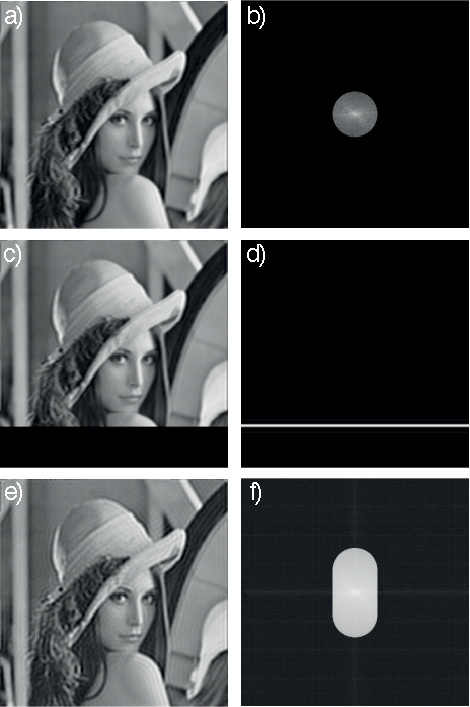
\includegraphics{widefield_slit}
  \caption{Simulation of a confocally scanned wide-field system or swept light-sheet system.
  a) Is the raw, image with b) showing Fourier space and the frequency passband.
  c) Shows a the confocal slit scanning in progress and d) shows what the SLM will be displaying.
  d) is the final image as it would appear after an acquisition and e) is the the new larger OTF is frequency space.
  }
  \label{fig:widefield_slit}
\end{figure}

\subsection{SIM}
High contrast fringes are needed to accurately reconstruct a SIM image.
To recover the $\mathbf{k}$ vectors in frequency space sharp peaks induced by the sinusoidal pattern are localised.
Contrast in real-space corresponds to SNR of these peaks.
%To reliably reconstruct a SIM image, high contrast fringes are needed to very accurately localise their points in Fourier space as fringe contrast in image space corresponds to the amplitude of the delta functions of a sinusoid in Fourier space..
If the localisation of these points is inaccurate, inverting the process of un-mixing the frequencies computationally will cause artefacts in the final image.
As discussed, slit scanning has the potential to increase image contrast without a sacrifice on speed of acquisition; to achieve this in SIM requires a very fast ferroelectric SLM.
As in the widefield case, a row of active pixels is swept during an exposure but now this pattern is the product of a standard set of SIM patterns (Fig. \ref{fig:sim_slit}).
For these simulations 9 patterns were used, 3 angles and 3 phases; though fewer can be used.

\begin{figure}
  \centering
  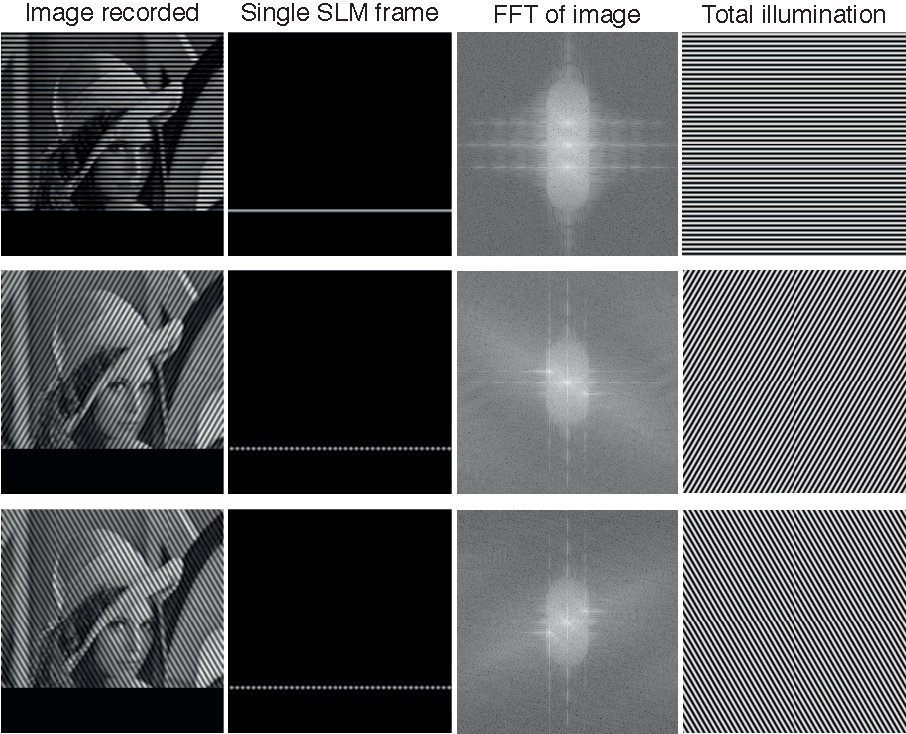
\includegraphics{sim_slit}
  \caption{a) Optical diagram for SLM implementation of dual-beam slit scanning.
           b) Diagram showing a much simplified approach for creating two beams optically with minimal los of photons, light-polarisation insensitivity and without the need for an SLM.}
  \label{fig:sim_slit}
\end{figure}

\subsection{mSIM}

For mSIM, During each exposure the SLM will display a single row illumination spots of the full lattice from a standard mSIM pattern.
This row is then swept synchronously with the virtual slit as before.
The act of using a virtual slit on the camera reduces the dimensionality of the reconstruction of an mSIM image, drastically increasing the speed of an acquisition without the need for additional optics.
Schroff \emph{et. al.}, for instance, require $200 \times 200$ images for a single mSIM reconstruction.
The proposed method here, would therefore increase the speed of this process by 200 fold.
This is dwarfed by iSIM, which gives instantaneous super-resolved images at the cost of requiring extensive optics.

\begin{figure}
  \centering
  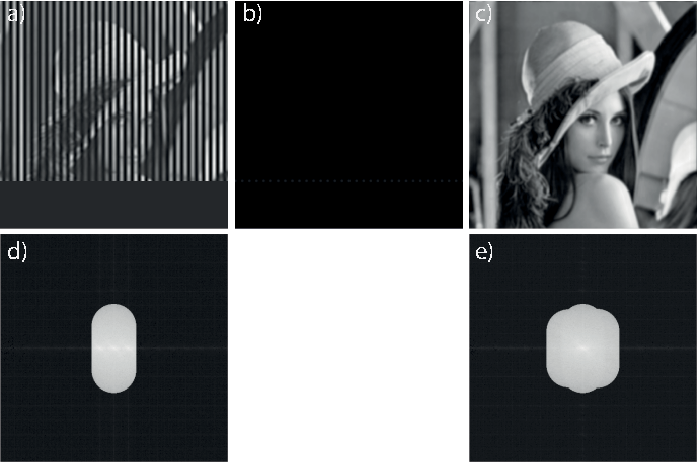
\includegraphics{msim_slit}
  \caption{
  a) The capturing of a single mSIM frame;
  b) mSIM illumination pattern as it rolls;
  c) reconstructed slit-mSIM image;
  d) OTF of a single mSIM frame;
  e) OTF of reconstructed slit-mSIM frame
  }
  \label{}
\end{figure}

Reconstructions for SIM were achieved using fairSIM.
fairSIM however assumes that each angle provided will have the same size OTF just rotated.
However, when using slit scanning the OTF support is large; as such fairSIM, though it reconstructs successfully, omits resolution in the $y$ direction.
For this work a custom reconstruction algorithm will be needed to maximise reconstruction reconstruction.

\section{Discussion}

It has been demonstrated that confocal slit scanning makes an improvement on SNR for recorded imaged.
This was characterised with beads.
however, imaging speeds using confocal slit scanning are half maximum when using a single beam.
to this end two beams were generated optically using a simple beam splitter and two mirrors.
Each beam could be independently positioned such that they were separated by a half a sensor area, at the camera plane.

\subsection{Simulations}

The effect of confocal slit scanning was explored \emph{in silico}, to verify the expectation that resolution and contrast could be improved using confocal slit scanning.
This was considered for orthogonally imaging systems, such as is light-sheet microscopy, but as well for epi-illumination systems with some degree of control over the structure of the illumination.
This would be realised by running an SLM at \SI{}{\kilo\hertz} rates, which is feasible for ferroelectric devices.
Initially slit scanning was considered for a flat illumination control across an image, and again it was found that a resolution increase could be attained.
Slit scanning was then applied to the, well-established, structured illumination techniques of SIM and mSIM.

\subsubsection{SIM}

Slit-scanned simulations of a test image were successfully reconstructed using fairSIM, an open source FIJI plugin (Fig. \ref{fig:sim_slit_reconstructed}).
It was expected that the contrast improvement in SIM would be the primary benefit to the technique.
However, it may be possible exploit the increase in resolution in one direction to increase the resolution of SIM further.
Currently fairSIM only considers possible OTF supports which have rotational symmetry.
The addition of confocal slit scanning means that, though the reconstruction is successful, higher resolution information afforded by slit scanning, is neglected.
Going further, it may be possible in a real system to display a very fine SIM pattern in the direction of confocal slit scanning.
The Moirè fringes of this image would ordinarily be blurred to the point where the SIM pattern in Fourier space would be outside of the passband.
Using slit scanning with SIM may allow the recovery of these fringes, for reconstruction, potentially giving up to a 4$\times$ resolution improvement, with better optical sectioning and contrast.

\begin{figure}
  \centering
  \includegraphics{sim_slit_reconstructed}
  \caption{slit-SIM images as reconstructed using fairSIM.
  a) The sum projected image of the 9 raw SIM images;
  b) with the complimentary Fourier space image, showing diffraction limited information in the horizontal.
  c) The slit-SIM reconstruction;
  d) with the Fourier space image showing how the OTF support, along the horizontal, has been extended beyond the diffraction limit.}
  \label{fig:sim_slit_reconstructed}
\end{figure}

\subsubsection{mSIM}

%Slit-scanning mSIm was considered whereby the number of images to be reconstructed in the final image was square-rooted.
Ordinarily, in mSIM, the virtual pin-holing step is achieved computational by reconstructing from an $n\times n$ set of images; using slit scanning the reconstruction reduces to $n$ only.
It was shown that the OTF of the reconstructed mSIM image continues to stretch in one direction up to 2 fold in the ideal.
Using fewer images should reduce the amount of time needed, but as slit-scanning does reject photons there may be a trade off in real samples when acquiring a sufficient number of photons to reconstruct an image.

\subsection{Future work}

\subsection{Dual slit scanning}

Confocal slit scanning can now be driven at full \SI{100}{\hertz} imaging rates and so could be applied to fast dynamic processes in need of contrast and axial resolution.
The intent with this work was to apply the improvement provided by slit-scanning to single particle tracking, as time resolution is essential for characterising motion; similarly a large field of FOV means particles can be tracked for longer times periods of time.
%allows for tracks to be recorded over longer epochs
An alternative manipulation having two independent chips is to chromatically separate channels onto each of the chips, for simultaneous two colour \SI{100}{\hertz} imaging.
Such image splitting devices do exist, with the trade-off of field of view for time-resolution.
Due to the additional optics added to the light-sheet system for the astigmatic tracking module, there was not sufficient space to investigate this technique further.

\subsection{Structured illumination slit scanning}

The simulations presented here can be immediately adapted onto microscope systems with SLMs already embedded, provided there is intensity (rather then phase) control at the sample plane.
For a 512$\times$512 px field of view, at \SI{40}{\milli\second} exposure, the SLM would need to be run at \SI{12.8}{\kilo\hertz} which is only viable for ferroelectric liquid crystal SLMs.
For slit-scanning-SIM to become valuable, a full rotational asymmetric reconstruction algorithm will need to be written which incorporates the potential one-directional resolution increase seen in the OTFs.

%a full dark state can be realised
%Dual slit work
%% Attempt in real samples, apply to virus tracking.
%Apple to real microscopes, should be a free upgrade as it is only computational.
% Calculate refresh rate for 512 px


%OTF has a funny shape
%Interestingly the OTF, in the direction that ungoes a post-processing reconstruction,

%future work, make an algorithm that works with SIM-slit-slit_scanning_alt

%Demonstrated that slit scanning does improvement
%The assumptions made here are that the imaging system is ideal, that imaging is only a frequency passband and that the axial is infinity thin.
%There exist adapters to split the image on the chip into two colours, could use slit scanning for that, though no room for tuning.
